\documentclass{beamer}
\usepackage[utf8]{inputenc}

\usetheme{Madrid}
\usecolortheme{default}
\usepackage{amsmath,amssymb,amsfonts,amsthm}
\usepackage{txfonts}
\usepackage{tkz-euclide}
\usepackage{listings}
\usepackage{adjustbox}
\usepackage{array}
\usepackage{tabularx}
\usepackage{lmodern}
\usepackage{circuitikz}
\usepackage{tikz}
\usepackage{graphicx}

\setbeamertemplate{page number in head/foot}[totalframenumber]

\usepackage{tcolorbox}
\tcbuselibrary{minted,breakable,xparse,skins}

% Background color for code boxes
\definecolor{bg}{gray}{0.95}
\DeclareTCBListing{mintedbox}{O{}m!O{}}{%
  breakable=true,
  listing engine=minted,
  listing only,
  minted language=#2,
  minted style=default,
  minted options={%
    linenos,
    gobble=0,
    breaklines=true,
    fontsize=\small,
    numbersep=8pt,
    #1},
  boxsep=0pt,
  left skip=0pt,
  right skip=0pt,
  left=25pt,
  right=0pt,
  top=3pt,
  bottom=3pt,
  arc=5pt,
  leftrule=0pt,
  rightrule=0pt,
  bottomrule=2pt,
  toprule=2pt,
  colback=bg,
  colframe=orange!70,
  enhanced,
  overlay={%
    \begin{tcbclipinterior}
    \fill[orange!20!white] (frame.south west) rectangle ([xshift=20pt]frame.north west);
    \end{tcbclipinterior}},
}

% Set listings settings for C language
\lstset{
    language=C,
    basicstyle=\ttfamily\small,
    keywordstyle=\color{blue},
    stringstyle=\color{orange},
    commentstyle=\color{green!60!black},
    numbers=left,
    numberstyle=\tiny\color{gray},
    breaklines=true,
    showstringspaces=false,
}

% Define command for column vector and bold vector letter
\newcommand{\myvec}[1]{\ensuremath{\begin{pmatrix}#1\end{pmatrix}}}
\renewcommand{\vec}[1]{\boldsymbol{#1}} % bold vectors

% Meta Info
\title{2.7.29}
\date{September, 2025}
\author{Mahesh Chollangi - EE25BTECH11017}

\begin{document}

\frame{\titlepage}

\section*{Question}
\begin{frame}{Question}
The area of a triangle formed by vertices $\vec{O}, \vec{A}$ and $\vec{B}$, where $\vec{OA} = \hat{i} + 2\hat{j} + 3\hat{k}$ and $\vec{OB} = -3\hat{i} - 2\hat{j} + \hat{k}$ is
\end{frame}

\begin{frame}{Solution}
Let \vec{O} be the origin

Represent the vectors in matrix form:
\begin{align}
\vec{A} = \myvec{1 \\ 2 \\ 3}, \quad
\vec{B} = \myvec{-3 \\ 1 \\ 1}
\end{align}

The area of triangle $OAB$ is given by:
\begin{align}
\text{Area} = \frac{1}{2} \norm{\vec{A} \times \vec{B}}
\end{align}

Compute the cross product using determinant:
\begin{align}
\vec{A} \times \vec{B} =
\myvec{
(2)(1) - (3)(1) \\
(3)(-3) - (1)(1) \\
(1)(1) - (2)(-3)
}
=
\myvec{
2 - 3 \\
-9 - 1 \\
1 + 6
}
=
\myvec{
-1 \\
-10 \\
7
}
\end{align}

\end{frame}

\begin{frame}{Solution}

Simplifying:
\begin{align}
\Rightarrow \vec{A} \times \vec{B} = \myvec{-1 \\ -10 \\ 7}
\end{align}

Magnitude of the cross product:
\begin{align}
\norm{\vec{A} \times \vec{B}} = \sqrt{(-1)^2 + (-10)^2 + 7^2} = \sqrt{1 + 100 + 49} = \sqrt{150}
\end{align}

Final area:
\begin{align}
\text{Area} = \frac{1}{2} \sqrt{150}
\end{align}

\end{frame}

\begin{frame}[fragile]
\frametitle{C code}
\begin{lstlisting}

#include <math.h>

double OA[3] = {1, 2, 3};
double OB[3] = {-3, -2, 1};

double cross_product[3];

// Function to compute cross product OA x OB
void compute_cross_product() {
    cross_product[0] = OA[1]*OB[2] - OA[2]*OB[1];
    cross_product[1] = OA[2]*OB[0] - OA[0]*OB[2];
    cross_product[2] = OA[0]*OB[1] - OA[1]*OB[0];
}

// Function to compute magnitude of cross product vector
double compute_area() {



\end{lstlisting}
\end{frame}


\begin{frame}[fragile]
\frametitle{C code}
\begin{lstlisting}

compute_cross_product();
    return 0.5 * sqrt(cross_product[0]*cross_product[0] +
                      cross_product[1]*cross_product[1] +
                      cross_product[2]*cross_product[2]);
}

\end{lstlisting}
\end{frame}

\begin{frame}[fragile]
\frametitle{Python code}
\begin{lstlisting}

import numpy as np
import matplotlib.pyplot as plt

# Define vectors OA and OB
OA = np.array([1, 2, 3])
OB = np.array([-3, -2, 1])

# Compute cross product
cross = np.cross(OA, OB)
area = 0.5 * np.linalg.norm(cross)

print(f"Area of triangle OAB = {area:.4f}")

# Plot the triangle vertices and edges
origin = np.array([0, 0, 0])


\end{lstlisting}
\end{frame}


\begin{frame}[fragile]
\frametitle{Python code}
\begin{lstlisting}

fig = plt.figure()
ax = fig.add_subplot(111, projection='3d')
# Plot points O, A, B
ax.scatter(*origin, color='black', label='O (0,0,0)')
ax.scatter(*OA, color='blue', label='A (1,2,3)')
ax.scatter(*OB, color='green', label='B (-3,-2,1)')

# Plot edges
ax.plot([origin[0], OA[0]], [origin[1], OA[1]], [origin[2], OA[2]], 'b')
ax.plot([origin[0], OB[0]], [origin[1], OB[1]], [origin[2], OB[2]], 'g')
ax.plot([OA[0], OB[0]], [OA[1], OB[1]], [OA[2], OB[2]], 'r')


\end{lstlisting}
\end{frame}


\begin{frame}[fragile]
\frametitle{Python code}
\begin{lstlisting}

ax.set_xlabel('X-axis')
ax.set_ylabel('Y-axis')
ax.set_zlabel('Z-axis')
ax.set_title(f'Triangle OAB with Area = {area:.4f}')
ax.legend()
plt.show()

\end{lstlisting}
\end{frame}

\begin{frame}{Plot}
    \begin{figure}[H]
    \centering
    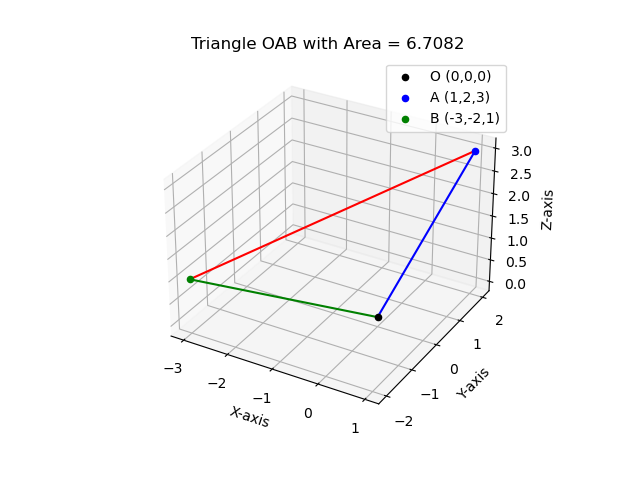
\includegraphics[width=0.8\columnwidth]{Figs/Figure_5.png}
    \caption{3D Plot}
    \label{3D Plot}
\end{figure}
\end{frame}

\end{document}
